%!TEX encoding = UTF-8 Unicode

\section{Experimental Results}

\subsection{GLU - Effect Prediction}

Our model permits to make predictions over the effects of actions onto environment objects.

In this experiment, we assume that the Gesture \acp{HMM} provide the discrete value of the recognized action performed by a human agent~(i.e., we enforce a hard decision over the observed action).
%, referring to the possible combination strategies listed in Sec.~\ref{sec:combination}).

\begin{figure}
    \centering
    \subfloat[][Prediction of the movement effect on a small sphere.]
    { 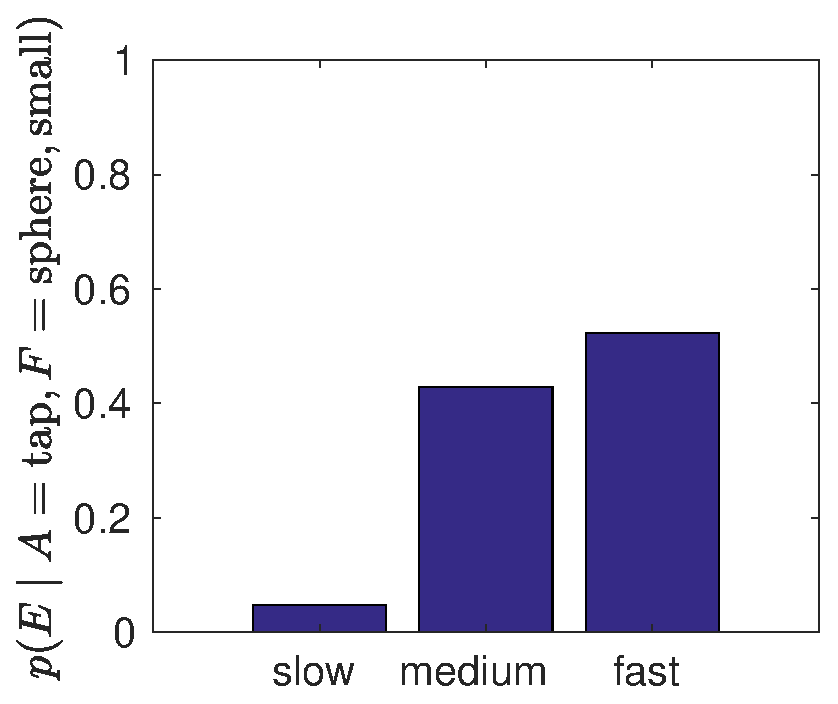
\includegraphics[width=0.45\linewidth]{effectpred_sphere.eps} \label{fig:effect_pred:sphere} } \quad
    %
    \subfloat[][Prediction of the movement effect on a big box.]
    { 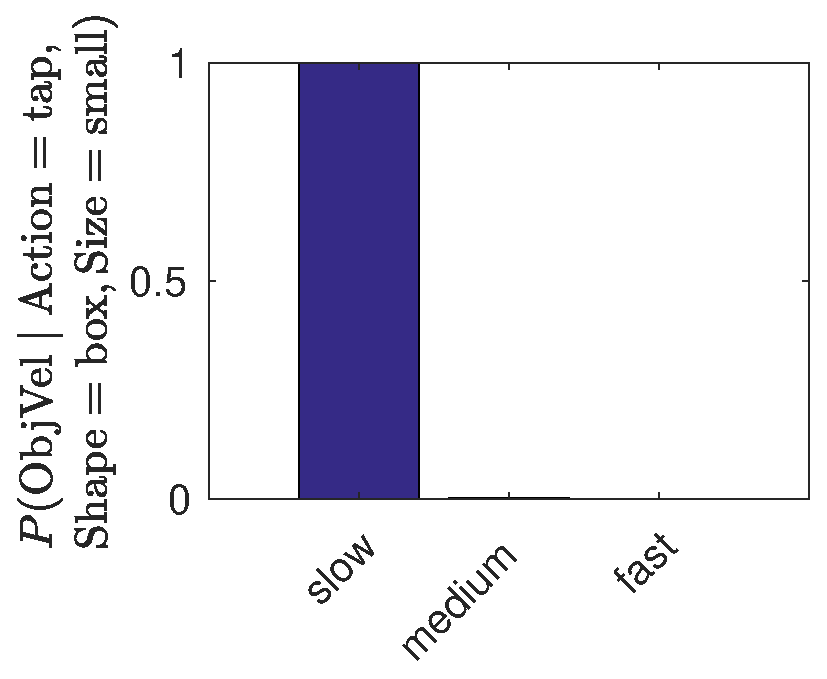
\includegraphics[width=0.45\linewidth]{effectpred_box.eps} \label{fig:effect_pred:box} }
    \caption{Object velocity predictions, given prior information~(from Gesture \acp{HMM}) that the human user performs a tapping action.}
    \label{fig:effect_pred}
\end{figure}


From our combined model of words, affordances and observed actions, we report the inferred posterior value of the Object Velocity effect, given prior information about the action~(provided by the Gesture \acp{HMM}) and also about object features~(Shape and Size). Fig.~\ref{fig:effect_pred} shows the computed predictions in two cases. Fig.~\ref{fig:effect_pred:sphere} shows the anticipated object velocity when the human user performs the tapping action onto a small spherical object, whereas Fig.~\ref{fig:effect_pred:box} displays it when the target object is a big box. Indeed, given the same observed action prior~(lateral tap on the object), the expected movement is very different depending on the physical properties of the target object.

\begin{figure}
\centering
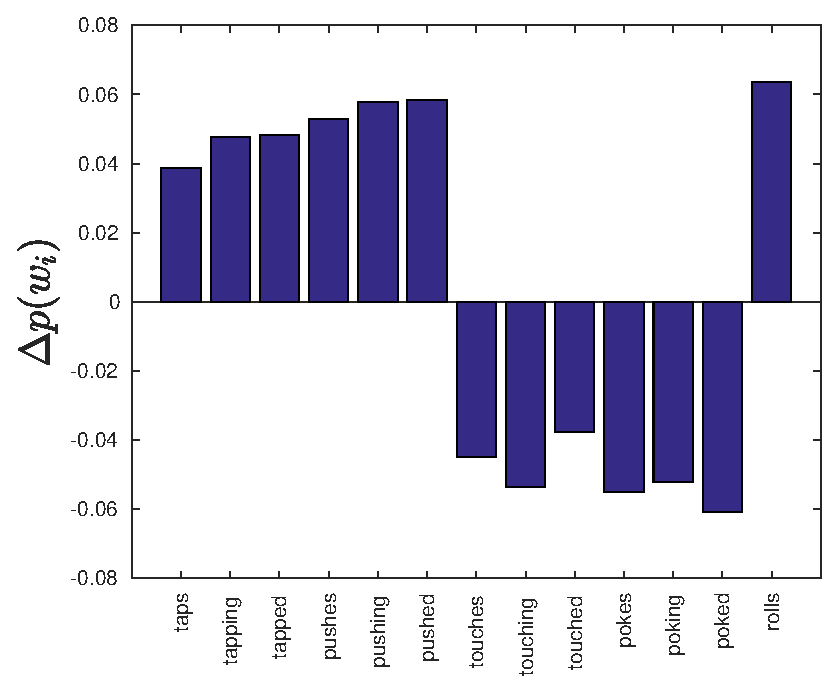
\includegraphics[width=0.9\columnwidth]{partialfig.eps}
\caption{Variation of word occurrence probabilities: $\Delta p(w_i) = p(w_i \mid F, E, A=\text{tap}) - p(w_i \mid F,E)$, where $F = \{\text{Size=big, Shape=sphere}\}$, $E = \{\text{ObjVel=fast}\}$. This variation corresponds to the difference of word probability when we add the tap action evidence~(obtained from the Gesture \acp{HMM}) to the initial evidence about object features and effects. We have omitted words for which no significant variation was observed.}
\label{fig:probdiff}
\end{figure}

\subsection{GLU - Prediction of Words}

Our model permits to make predictions over the associated word descriptions in the presence or absence of an action prior.

As in the previous experiment, we assume that the Gesture \acp{HMM} provide the discrete value of the recognized action performed by a human agent~(i.e., we enforce a hard decision over the observed action).

We compare the associated \emph{verbal description} obtained by the \acl{BN} in the absence of an action prior, with the ones obtained in the presence of one. In particular, we compare the \emph{probability of word occurrence} in the following two situations:
\begin{enumerate}
\item when the robot prior knowledge~(evidence in the \ac{BN}) includes information about object features and effects only: \emph{Size=big, Shape=sphere, ObjVel=fast};

\item when the robot prior knowledge includes, in addition to the above, evidence about the action as observed from the Gestures \acp{HMM}: \emph{Action=tap}.
\end{enumerate}

Fig.~\ref{fig:probdiff} shows the variation in word occurrence probabilities between the two cases, where we have omitted words for which no significant variation was observed in this case. We can interpret the difference in the predictions as follows:
\begin{itemize}
\item as expected, the probabilities of words related to tapping and pushing increase when a tapping action evidence from the Gestures \acp{HMM} is introduced; conversely, the probabilities of other action words~(touching and poking) decreases;

\item interestingly, the probability of the word \emph{rolling}~(which is an effect of an action onto an object) also increases when the tapping action evidence is entered. Even though the initial evidence of case~$1$ already included some effect information~(the velocity of the object), it is only now, when the robot perceives that the physical action was a tap, that the event rolling is associated.
\end{itemize}

\subsection{Emergence of Verbal Descriptions}

In the previous experiment, we have seen how our model is able to generate word probabilities after having received probabilistic observed evidence.
In order to illustrate the capabilities of the model, we use the \ac{CFG} described in Appendix~\ref{appendix:grammar} to generate written descriptions of the robot observations on the basis of the probability distributions of the words inferred by the model.
Note that this grammar is defined here with the only purpose to interpret the probability distributions over the words.
The grammar was neither used in the speech recognition system, nor in learning the associations of the spoken utterances to the affordance variables.
In the model described in~\cite{salvi:2012:smcb}, the speech recognizer used a free loop of words with uniform prior distribution over the words, and the Bayesian model used a bag-of-words assumption, thus disregarding any syntactic information about the spoken descriptions.

%Before analyzing the results, some clarifications are due about the \ac{CFG}:
%(i)~this grammar was used only for automatic speech recognition of the spoken descriptions provided by human narrators in the experiment of~\cite{salvi:2012:smcb}; it was \emph{not} used during the \AffWords{} \ac{BN} learning phase, which was unsupervised;
%(ii)~the speech recognizer is based on the bag-of-words assumptions, meaning that it considers a loop of words with no grammatical structure, where only the binary presence or absence of each word is considered;
During the self-centered learning phase, the verbal descriptions described the agent of the observed actions as either ``the robot'', ``he'', or ``Baltazar''.
Consequently, the \AffWords{} model learned by the robot includes those words.
In the current study, by merging the \AffWords{} model and the gesture/action recognition model, we allow the robot to reinterpret the concepts it has learned in the self-centered phase, but we do not add any new words to the model.
Consequently, the descriptions that the model generates when observing humans use the same words to describe the agent.

%The first expression of sentences formed with the grammar is always a subject with the non-terminal token \verb!<agent>!, which is expanded \emph{randomly} to one of the following: ``the robot'', ``he'', or ``Baltazar''~(i.e., the name of the humanoid robot used in the experiments). In other words, the choice of the possible expansion is not related to the evidence in the other nodes of the model. This is evident also by looking at the leftmost word nodes of Fig.~\ref{fig:grammar}, which not linked to any other words.

The textual descriptions are generated as follows: we provide evidence to the model~(hard or soft evidence), we extract the generated word probabilities $P(w_i\given \text{evidence})$.
We generate $N$ sentences randomly from the \ac{CFG} using the \texttt{HSGen} tool from HTK~\cite{young:htkbook}.
Then, the sentences are re-scored according to the log-likelihood of each word in the sentence, normalized by the length of the sentence:
\begin{equation*}
  \text{score}(s_j\given \text{evidence}) = \frac{1}{n_j} \sum_{k=1}^{n_j} \log P(w_{jk}\given \text{evidence}),
\end{equation*}
where~$s_j$ is the~$j$th sentence,~$n_j$ is the number of words in the sentence~$s_j$, and~$w_{jk}$ is the~$k$th word in the sentence~$s_j$.

Finally, an $N$-best list of possible descriptions is produced by sorting the scores.

%To examine the generated verbal description, we proceed as follows:  and then we match them to a list of~\SI{1000} possible sentences~(randomly generated according to the \ac{CFG}).
%The matching process is described in Appendix~\ref{appendix:grammar}.

For example, if we provide the following evidence the model:
\begin{equation*}
\{\text{Color=yellow, Size=big, Shape=circle, ObjVel=fast}\},
\end{equation*}
we obtain the sentences reported in Table~\ref{tab:generated_sentences_1}.

\begin{table}
    \centering
    \caption{Sentences generated from the evidence $\{\text{Color=yellow, Size=big, Shape=circle, ObjVel=fast}\}$. The higher the score, the better. In the most likely sentence, the correct action-related verb ``taps'' is generated, and the object term ``ball'' is used twice, both in the first part and in the second part of the sentence.}
    \label{tab:generated_sentences_1}
    \begin{tabular}{ll}
    \toprule
    sentence & score \\
    \midrule
    \textbf{baltazar tapped the ball and the ball moves} & \bm{$-0.63813$} \\
    baltazar taps the ball and the sphere is moving & $-0.64636$ \\
    the robot touched the big sphere and the ball is rolling & $-0.64822$ \\
    he taps the sphere and the sphere moves & $-0.65437$ \\
    the robot has poked the ball and the sphere moves & $-0.67455$ \\
    baltazar just tapped the sphere and the sphere is rolling & $-0.71942$ \\
    baltazar taps the sphere and the big ball rolls & $-0.72702$ \\
    baltazar taps the sphere and the yellow sphere rolls & $-0.73154$ \\
    the robot just touched the sphere and the ball moves & $-0.79609$ \\
    baltazar has poked the ball and the ball rolls & $-0.81551$ \\
    \bottomrule
    \end{tabular}
\end{table}

\subsection{Reasoning over Effects, Choice of Correct Conjunction}

Example in which the generated conjunction is ``and'' (because of consistency between Action, Object Features and Effect evidence):

evidence: \emph{\{'Size', 'small', 'Shape', 'box', 'Action', 'touch', 'Contact', 'long', 'ObjHandVel', 'slow'\}}

resulting word probabilities: Fig.~\ref{fig:conjunction_and:pw}

\begin{figure}
\centering
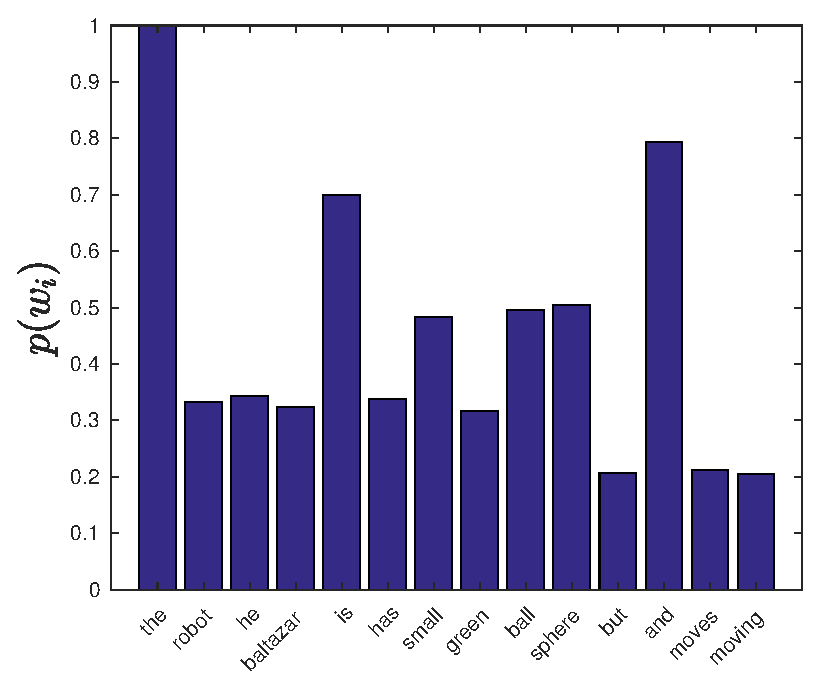
\includegraphics[width=0.9\columnwidth]{and_pw.eps}
\caption{Word occurrence probabilities given the evidence \emph{\{'Size', 'small', 'Shape', 'box', 'Action', 'touch', 'Contact', 'long', 'ObjHandVel', 'slow'\}}. We have omitted words for which no significant probability was observed.}
\label{fig:conjunction_and:pw}
\end{figure}

generated sentences in Tab.~\ref{tab:conjunction:and}

\begin{table*}
    \centering
    \caption{.}
    \label{tab:conjunction:and}
    \begin{tabular}{ll}
    \toprule
    sentence & score \\
    \midrule
    the robot has touched the box and the square is still & $-0.55989$ \\
    the robot is touching the box and the blue square is inert & $-0.62944$ \\
    the robot has poked the green box and the yellow box is inert & $-0.68388$ \\
    baltazar is touching the blue box and the square is still & $-0.69946$ \\
    baltazar has poked the cube and the yellow box is inert & $-0.71426$ \\
    baltazar touched the yellow cube and the square is still & $-0.72961$ \\
    the robot pokes the yellow square and the yellow cube is inert & $-0.73993$ \\
    the robot has just touched the yellow box and the square is inert & $-0.76648$ \\
    baltazar pokes the green square and the blue box is still & $-0.80106$ \\
    he just poked the blue cube and the yellow cube is still & $-0.97389$ \\
    \bottomrule
    \end{tabular}
\end{table*}

Example in which the generated conjunction is ``but'' (because of no consistency):

evidence: \emph{\{'Size', 'small', 'Shape', 'box', 'Action', 'touch', 'Contact', 'short', 'ObjHandVel', 'medium'\}}

resulting word probabilities: Fig.~\ref{fig:conjunction_but:pw}

\begin{figure}
\centering
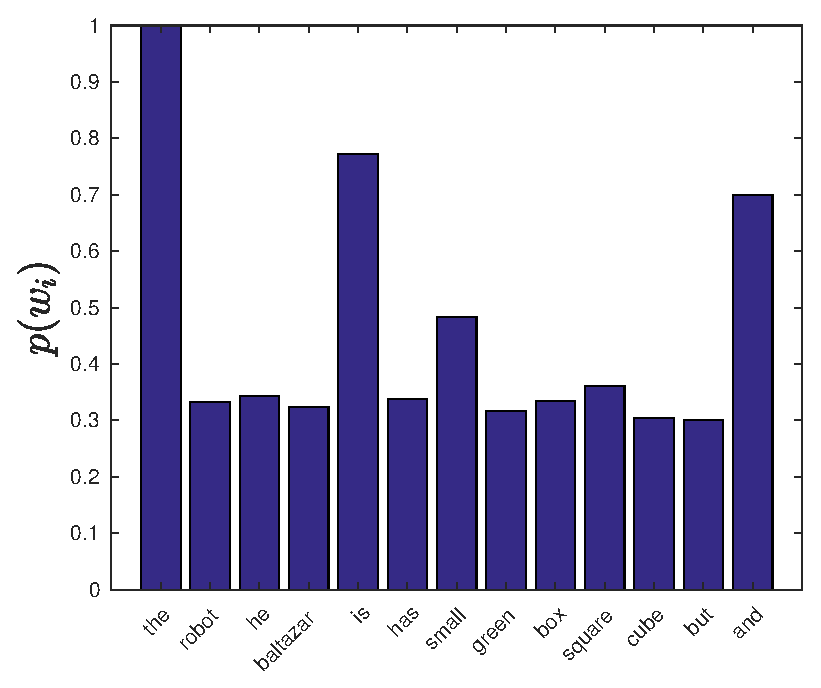
\includegraphics[width=0.9\columnwidth]{but_pw.eps}
\caption{Word occurrence probabilities given the evidence \emph{\{'Size', 'small', 'Shape', 'box', 'Action', 'touch', 'Contact', 'short', 'ObjHandVel', 'medium'\}}. We have omitted words for which no significant probability was observed.}
\label{fig:conjunction_but:pw}
\end{figure}

generated sentences in Tab.~\ref{tab:conjunction:but}

\begin{table*}
    \centering
    \caption{.}
    \label{tab:conjunction:but}
    \begin{tabular}{ll}
    \toprule
    sentence & score \\
    \midrule
    the robot is touching the cube but the square is inert & $-0.69236$ \\
    the robot is poking the square but the cube is rolling & $-0.70946$ \\
    he is touching the green box and the box is moving & $-0.71492$ \\
    the robot has touched the box and the square is still & $-0.72471$ \\
    he is touching the square but the small square is inert & $-0.74044$ \\
    the robot has touched the green square and the small box is moving & $-0.74836$ \\
    the robot just poked the small square but the square is moving & $-0.8005$ \\
    the robot is touching the box and the blue square is inert & $-0.80153$ \\
    the robot is poking the box and the blue square is moving & $-0.80337$ \\
    baltazar is touching the box but the box moves & $-0.807$ \\
    \bottomrule
    \end{tabular}
\end{table*}

\subsection{Solving Ambiguities with the Combined Model}

Fig.~\ref{fig:update_from_softevidence} shows the result of predictions over nodes given some (hard) evidence, before and after incorporating further soft evidence

\begin{figure*}
    \centering
    \subfloat[][Prediction of the model given the initial (hard) evidence.]
    { 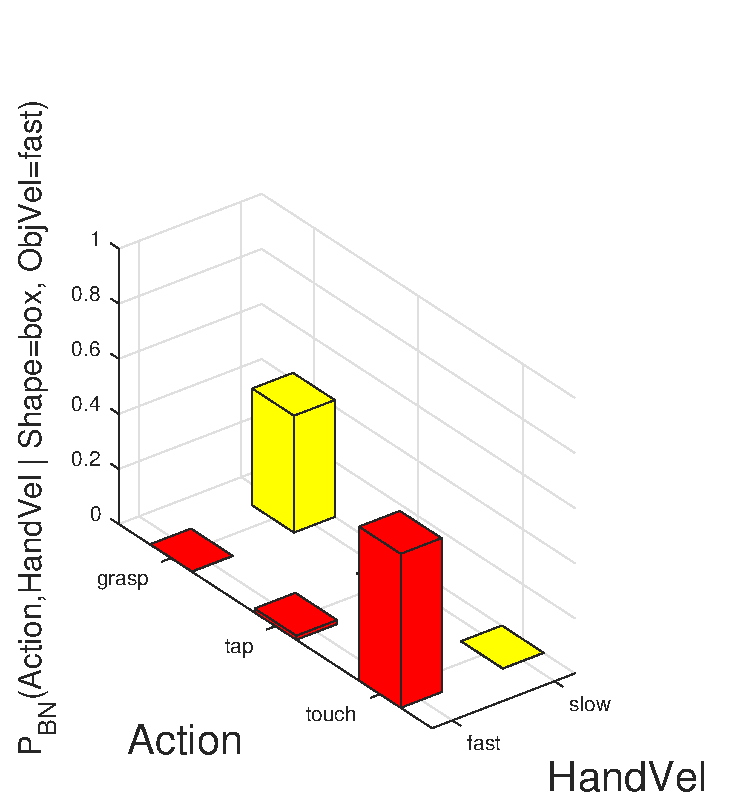
\includegraphics[width=0.45\linewidth]{before_softevidence_prediction.eps} \label{fig:before_softevidence:pred} } \quad
    %
    \subfloat[][Updated prediction of the model after having incorporated the Action soft evidence.]
    { 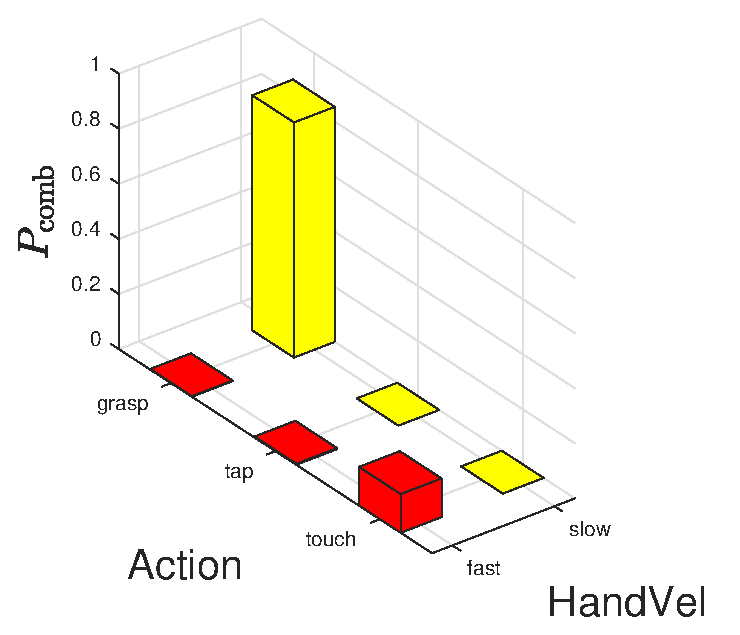
\includegraphics[width=0.45\linewidth]{after_softevidence_prediction.eps} \label{fig:after_softevidence:pred} }
    \caption{.}
    \label{fig:update_from_softevidence}
\end{figure*}

word probabilities: Fig.~\ref{fig:after_softevidence:pw} (right now they are identical before and after incorporating the soft evidence)

\begin{figure}
\centering
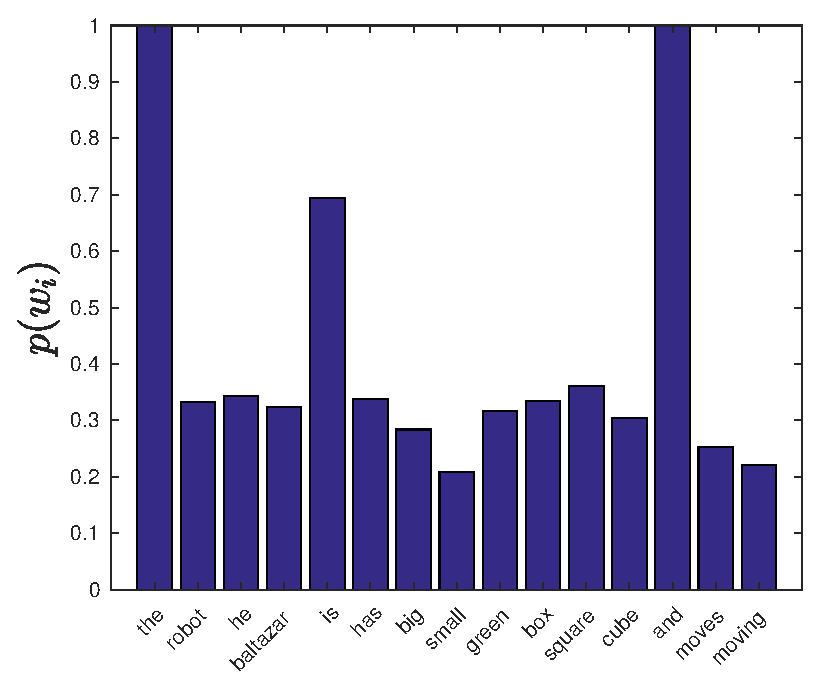
\includegraphics[width=0.9\columnwidth]{after_softevidence_pw.eps}
\caption{Word occurrence probabilities given the evidence \emph{\{'Shape', 'box', 'ObjVel', 'fast'\}}. We have omitted words for which no significant probability was observed.}
\label{fig:after_softevidence:pw}
\end{figure}
